\subsection{Goodness of fit tests}
So far we have mostly discussed comparing one hypothesis against another for the purposes of making decisions / choosing between them. However, what if we wanted to just compare the data to a particular hypothesis and make a statement about whether or not the distribution used to describe the data is suitable or not. This problem falls under the class of tests called \emph{goodness of fit tests}. We won't go into detail here as there are many different goodness of fit tests available which are sensitive to different features in the data. Some are good at spotting poor description in the tails of distributions and some are better for giving an overall impression of the agreement. Instead, let's focus on one goodness of fit test which provides another use of ratios of likelihoods. 

Suppose we have a histogram of data and a histogram (either derived from some analytic function or from MC simulation) describing what we expect to see under some hypothesis. We can ask how well the hypothesis agrees with that data. Each bin in the histogram can be thought of as an independent Poisson random process. The observed number of events in each bin is labelled $o_{i}$ and the expected (Poisson mean) values are $\lambda_{i}$. The likelihood function is then the product over Poisson probability distributions, 
\begin{equation}
    L(H_0) = \prod_{i} (\lambda_{i})^{o_{i}}e^{-\lambda_{i}}.
\end{equation}
Note that we've ignored the $o_{i}!$ terms, since in the end, this constant will drop out of the ratio of likelihoods. 

We haven't specified an alternate hypothesis, but there is something we can use. The so called \emph{saturated model} is the one for which the \emph{maximum likelihood} is achieved for any values of the $\lambda_{i}$. This is usually not a physics motivated hypothesis, but can be seen as the ``best'' hypothesis given the data, since its the hypothesis that exactly matches the data -- i.e $\lambda_{i}=o_{i}$ is the saturated model which yields our alternate hypothesis $H_1$. We then have, 
\begin{equation}
    \Lambda = \frac{L(H_0)}{L(H_1)} = \frac{\prod_{i} (\lambda_{i})^{o_{i}}e^{-\lambda_{i}}}{\prod_{i} (o_{i})^{o_{i}}e^{-o_{i}}}.
\end{equation}
In our previous example, the values of the likelihood function were $\mathcal{O}(1)$, however if we have many bins, these values will start to get very very small and hence numerically difficult. A common solution in HEP is to instead take the natural log of the likelihood - in fact (for reasons that will become clear later), we usually take $-2\times$ the log of the likelihood. The product becomes a sum, and we have, 
\begin{equation}
    -2\ln\Lambda = -2\ln\frac{L(H_0)}{L(H_1)} = -2\sum_{i} \left(o_{i}\ln(\lambda_{i}) -\lambda_{i}-o_{i}\ln(o_{i}) +o_{i} \right)
\end{equation}
 \begin{tcolorbox}[colback=backblue]
\textbf{Example:} Suppose we measure the energy of outgoing particles that scatter off a target. We know their incoming energy and hence we measure the distribution of the fraction of that energy which is carried away by the scattered particle. Let the energy fraction be $x\in[0,1]$ and our hypothesis for the distribution is an exponential with slope parameter -2, 
\begin{equation}
f(x)=Ne^{-2\cdot x}, ~N=2(1-e^{-2})^{-1} \approx 2.313
\end{equation}
We bin the observable $x$ into 5 equal width bins in the range $[0,1]$ and count the number of events that fall into each bin. We observe the following counts in the data 9,  6,  4,  5 and 2. Given $H_0$, the expected counts can be determined as $\lambda_{i}  =  26\times\int_{x_{a_{i}}}^{x_{b_{i}}}f(x)dx$, where $[x_{a_{i}},x_{b_{i}}]$ defines the boundaries of bin $i$ and we've observed 26 events in total.  Plugging in our observation, we see a value of $-2\ln\Lambda=1.32$. We can calculate the distribution of $-2\ln\Lambda$ and hence a $p$-value of 0.935. The code below is an example of how to do this using MC simulation, and the output is shown in Figure~\ref{fig:gof}.
\begin{lstlisting}[style = Python]
import numpy
from scipy.stats import poisson
import matplotlib.pyplot as plt
plt.rcParams.update({'font.size': 14})

# observed counts in each bin - norm is what we'll use to obtain lambdas
bin_boundaries = [0 , 0.2, 0.4, 0.6, 0.8, 1]
observations   =  [ 9,  6,  4,  5,  2 ]
norm = sum(observations)

# define a log function to handle 0 - will be 0 by the product
def mlog(o):
  if o==0: return 0
  else: return numpy.log(o)

# define the goodness of fit test likelihood ratio
def neg2logLambda(observations,lambdas):
  return -2*sum([o*mlog(l) - l - o*mlog(o) + o \
    for o,l in zip(observations,lambdas)])

# calculate the Poisson parameter for a given bin
# the bin is defined by the range x0->x1
a=2.0
def mean_exp(x0,x1):
  N = a*(1-numpy.exp(-a))**-1
  return (N/a)*(numpy.exp(-a*x0)-numpy.exp(-a*x1))

lambdas = [norm*mean_exp(x,x+0.2)  for x in bin_boundaries[0:-1]]
test_stat_obs = neg2logLambda(observations,lambdas)

# generate the distributuon of the test stat under our hypothesis
test_stat_toys = []; pval = 0
for i in range(50000):
  toy_observations = [numpy.random.poisson(l) for l in lambdas]
  test_stat_t = neg2logLambda(toy_observations,lambdas)
  test_stat_toys.append(test_stat_t)
  if test_stat_t > test_stat_obs : pval += 1
pval/=len(test_stat_toys)

print("-2ln Lambda = ",test_stat_obs, ", p-value = ", pval)

# plot the data, and the exponential hypothesis
xaxis = numpy.arange(0,1,0.01); fig, (ax1,ax2) = plt.subplots(1,2)

ax1.plot([b+0.1 for b in bin_boundaries[0:-1]],observations,\
    marker="o",color="black", linestyle='none')
ax1.plot([b+0.1 for b in bin_boundaries[0:-1]],\
    lambdas, marker="_",color="red",linestyle='none')

ax2.hist([t for t in test_stat_toys if t > 1.3], \
    bins=numpy.arange(0,16,0.1),range=(0,16),color='cyan')
ax2.hist(test_stat_toys, bins=numpy.arange(0,16,0.1), \
    range=(0,16),color='black',histtype='step')
ax2.plot([test_stat_obs,test_stat_obs],[0,20],color='red')

ax1.set_xlabel("$x$"); ax1.set_ylabel("Observed/Expected events per bin")
ax2.set_xlabel("$-2\ln\Lambda$"); ax2.set_ylabel("# entries")
plt.show()
\end{lstlisting}
\end{tcolorbox}

\begin{figure}
    \centering
    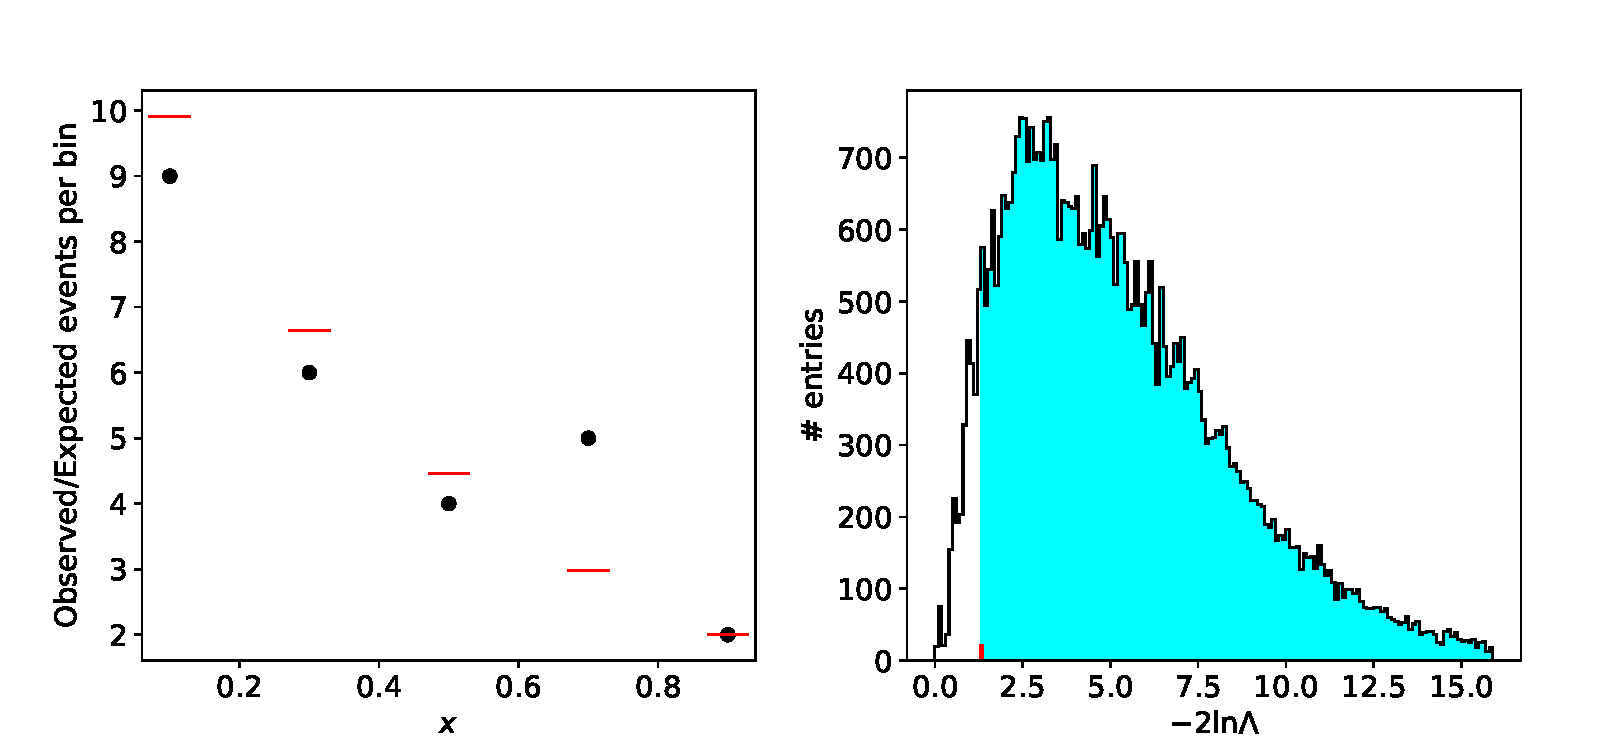
\includegraphics[width=\textwidth]{figures/Hypotest/gof_ex.pdf}
    \caption{Goodness of fit test for an exponential hypothesis ($H_0$) using the saturated model as the alternate hypothesis ($H_1$). The left plot shows the distribution observed in data (black markers) and the expectation under $H_0$ (red markers), while the right shows the distribution of $-2\ln\Lambda$ under $H_0$ (black histogram) and the observed value (red line). The cyan histogram shows the region integrated to calculate the $p$-value. }
    \label{fig:gof}
\end{figure}

In our example, we had to calculate the distribution of the test-statistic in order to calculate the $p$-value. One of the practical benefits of likelihood ratios, is their asymptotic properties. As you will show in your problems, the Poisson distribution will converge to a Gaussian distribution as $\lambda\rightarrow\infty$. Figure~\ref{fig:gof_cf_chi2} shows the distribution of $-2\ln\Lambda$ for the same exponential function example, scaling the number of expected events in each bin by a factor of 3 and 50. 

\begin{figure}
    \centering
    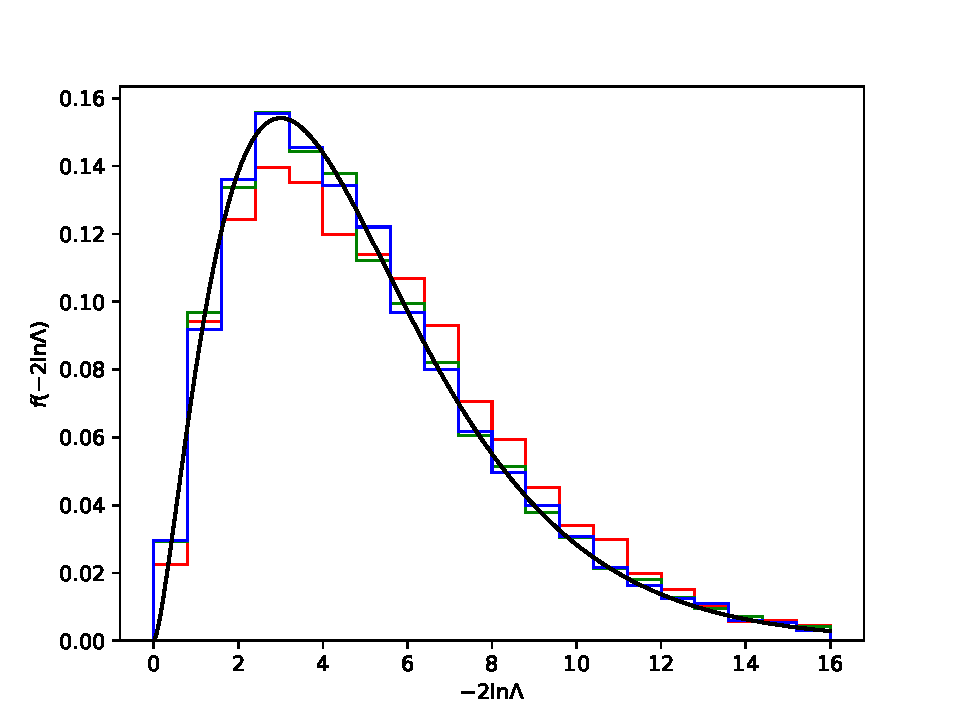
\includegraphics[width=0.8\textwidth]{figures/Hypotest/gof_cf_chi2.pdf}
    \caption{Distribution of $-2\ln\Lambda$ where the expected number of events in each bin ($\lambda_{i}$) under $H_0$ are scaled by 1 (red), 3 (green) and 50 (blue). A $\chi^{2}$ probability density function with 5 degrees of freedom (black line) is shown for comparison.}
    \label{fig:gof_cf_chi2}
\end{figure}

If we scale the number of expected events by 3 or 50, we start to see that the distribution of $-2\ln\Lambda$ doesn't change very much. In fact, it tends towards a well known distribution -- the $\chi^{2}$ probability density with 5 degrees of freedom. This is not surprising and is a consequence of Wilkes' theorem. We will come back to this later but you should keep in mind that very often, we in HEP look for test statistics that have known distributions in the asymptotic (large numbers) limit. This makes calculations of $p$-values (and hence as we'll see upper limits and confidence intervals) for the frequentist paradigm very efficient since we can usually avoid MC simulations, provided we are dealing with large numbers. Before we go onto discussing the test statistics which are used widely in HEP for setting limits and measuring quantities, we need to introduce a new concept -- \emph{nuisance parameters}.
